\documentclass[a4paper,12pt,numbered,oneside,openany]{uathesis}
\usepackage{graphicx}
\usepackage{cmap}
\usepackage{amssymb}
\usepackage{amsmath}
\usepackage{setspace}
\usepackage{booktabs}
\usepackage{url}
\usepackage{adjustbox}
\usepackage{tabularx}
\usepackage{multicol}
\usepackage{listings}
\usepackage{subcaption}
\usepackage[inline]{enumitem}
\usepackage[table,usenames,dvipsnames]{xcolor}
\usepackage{tikz}
\usetikzlibrary{positioning}
\usepackage{cleveref}
\usepackage{makecell}
\usepackage[acronym]{glossaries}
\usepackage{glossary-mcols}
\renewcommand*{\glspostdescription}{}
\renewcommand{\glossarypreamble}{\vspace*{-4em}}

\usepackage[Lenny]{fncychap}
\ChNameVar{\fontsize{18}{20}\usefont{OT1}{ptm}{m}{n}\selectfont}
\ChTitleVar{\huge\bfseries\fontfamily{ptm}\selectfont}
\usepackage{titlesec}

\newtheorem{definition}{Definition}
\newcolumntype{Y}{>{\centering\arraybackslash}X}
\renewcommand\floatpagefraction{.9}
\renewcommand\topfraction{.9}
\renewcommand\bottomfraction{.9}
\renewcommand\textfraction{.1}
\setcounter{totalnumber}{50}
\setcounter{topnumber}{50}
\setcounter{bottomnumber}{50}

\definecolor{light-gray}{gray}{0.95}
\newcommand{\code}[1]{\colorbox{light-gray}{\texttt{#1}}}
% Placeholder for numbers or text that depend on experiments still running.
\newcommand{\todo}[1]{\textcolor{red}{[TODO: #1]}}

\lstset{basicstyle=\ttfamily\small,breaklines=true,frame=single,columns=fullflexible}

\newlist{questions}{enumerate}{2}
\setlist[questions,1]{label=\textit{RQ\arabic*.},ref=\textit{RQ\arabic*}}
\setlist[questions,2]{label=(\alph*),ref=\thequestionsi(\alph*)}

\renewcommand{\figurename}{Figure}

\makeglossaries
\loadglsentries{glossary}

\begin{document}
\title{Learning from Earlier Websites: Cross-Task Long-Term Memory for a Small Website-Generation Model}
\author{Qiaopan Ma}
\subjectarea{Artificial Intelligence}
\dept{School of Computer Science}
\supervisor{Qian Liu}
\crest{
\includegraphics[width=0.2\textwidth]{University_of_Auckland_Coat_of_Arms.png}}
\degreetitle{Master of Artificial Intelligence}
\degreedate{2026}
\university{The University of Auckland}

\maketitle

\frontmatter
\begin{abstract}
Large language model (LLM) agents that generate websites solve every task from scratch: what went wrong on one website is forgotten before the next one starts. This dissertation asks whether a \emph{small} generator, the 7-billion-parameter WebGen-LM-7B, can improve across a sequence of WebGen-Bench tasks if it is given a long-term memory built from its own earlier attempts, without changing its weights or the official evaluation protocol.

We first reproduce the official No Memory baseline on a self-hosted cluster (28.5\% accuracy on 101 tasks versus 28.4\% reported). An analysis of its failures shows that most zero-score tasks are not hard tasks but blank pages caused by basic code errors, such as importing a package that is not installed, and that the model rarely follows advice written as text. A first text-based memory therefore helps early in the sequence but falls behind No Memory later, as generic advice accumulates in the prompt.

The final design (v7) combines three parts: a requirement checklist that keeps every requested feature visible; a code pool that, once a problem has appeared in at least two tasks, injects a short verified code fragment taken from the chain's own successful websites; and memory hygiene through deduplication at storage time, a concreteness filter and utility-based retirement. In a single run over all 101 tasks, v7 reaches 40.0\% accuracy against 28.5\% for No Memory (mean paired gain 11.5 points, 95\% CI 6.0--16.9) and reduces zero-score tasks from 30 to 13; unlike a text-only memory, its advantage holds over the last 71 tasks (40.4\% vs 29.5\%). Gains are functional: appearance on sites that work is unchanged. \todo{Add ablation and task-order results.}

The main lesson is that, for a small generator, \emph{what form} a memory takes matters more than how much is remembered: verified code fragments transfer where textual lessons do not. We discuss the limits of these single-run results, the cost of the evaluation, and the ethical considerations of self-improving code agents.
\end{abstract}

\begin{acknowledgements}
First and foremost, I would like to express my sincere gratitude to my supervisor, Dr Qian Liu, for supervising this project, for giving me the freedom to pursue a research direction I cared about, and for the support, encouragement and opportunities to present and discuss the work at group meetings. I am grateful for the trust and the research environment provided throughout this year.

I am also deeply grateful to Ziqin Zhu, a PhD student in Dr Liu's group, for generous guidance on how to do research and how to write it up: how to frame research questions, design fair experiments, and structure a dissertation. This advice shaped much of the way this work was carried out and written.

I also thank Tanya Carter, the programme manager of the Master of Artificial Intelligence, for coordinating the research project course, including the supervision arrangements.

I am grateful to the School of Computer Science at the University of Auckland for access to the CS ML GPU cluster. All experiments in this dissertation were run on its NVIDIA H200 GPUs; without this resource, running more than a thousand website generations with self-hosted models would not have been possible.

Finally, I thank my family for their support.

\begin{flushright}
Qiaopan Ma

November, 2026
\end{flushright}
\end{acknowledgements}

\setcounter{tocdepth}{1}
\tableofcontents
\addtocontents{toc}{\vspace{-4em}}
\listoffigures
\addtocontents{lof}{\vspace{-4em}}
\listoftables
\addtocontents{lot}{\vspace{-4em}}
\printglossary[type=\acronymtype, style=mcolindex, nonumberlist]

\mainmatter
\chapter{Introduction}
\label{chap:intro}
\glsresetall

\section{Background}
\subsection{Website Generation with Language Models}
Agents built on \glspl{llm} can now turn a natural-language request into a running website~\cite{lu2025webgenbench}. A user describes the pages and features they need, for example a booking form, a product list and a contact page, and the agent writes a complete project, installs its dependencies and starts it. Benchmarks such as WebGen-Bench evaluate this ability end to end: the generated project is started, and a \gls{vlm} tester clicks through the site to check whether each requested feature actually works~\cite{lu2025webgenbench,he2024webvoyager}. This is a demanding test. A website that looks plausible in a screenshot but has a form that does nothing, or a page that cannot be reached from the navigation, fails the corresponding check.

The strongest results on such benchmarks come from large proprietary models. Small open models are attractive for a different reason: they can be run locally, at low cost and without sending data to a third party. WebGen-LM-7B, the 7-billion-parameter generator released with WebGen-Bench, was fine-tuned specifically for this task, yet it reaches only 28.4\% accuracy under the official protocol~\cite{lu2025webgenbench}. Improving small generators without retraining them is therefore a practical problem as well as a research one.

\subsection{Every Task Is Solved in Isolation}
In WebGen-Bench, as in most code-generation benchmarks, every task is solved independently. The agent starts each task with the same weights and the same empty context. An agent that produced a blank page on one task because it imported a package that was not installed will make the same mistake on the next task, and on the one after that. In our reproduction of the baseline (\Cref{sec:nm-failures}), almost a third of the 101 tasks received a score of zero, and many of these failures had the same few causes: an undeclared dependency, a missing import, or a template that does not compile.

Human developers do not work this way. A developer who has broken a build once remembers why, and the second time the same situation appears they avoid it. The failures above are exactly the kind of mistakes that experience should remove.

\subsection{Long-Term Memory for Agents}
Recent work on agent memory tries to give \glspl{llm} this ability. After each task, the agent reflects on its trajectory, stores lessons or reusable procedures, and retrieves the relevant ones when it meets a later task~\cite{zhao2024expel,wang2023voyager,reasoningbank2025,wang2025awm,dai2026metis}. These systems report clear gains, but almost all of them use large, capable models as the agent. The memory is usually stored as natural-language insight, and the agent is trusted to understand and apply it.

It is much less clear whether the same approach works for a \emph{small} model. Small models follow long or numerous instructions less reliably~\cite{harada2025curse,jaroslawicz2025ifscale,li2025smallmodels}, are easily distracted by irrelevant context~\cite{shi2023distracted}, and degrade as the prompt grows even when all of it is relevant~\cite{du2025contextlength,liu2024lost}. A memory that adds a paragraph of lessons to every prompt may therefore help a large model and hurt a small one. Which \emph{form} of memory a small model can actually use is an open question.

\section{Problem Statement}
This dissertation asks whether a small website generator can get better with experience, without any change to its weights. We study the question on WebGen-Bench with WebGen-LM-7B. The generator, the agent scaffold (Bolt.diy) and the official evaluation protocol are kept fixed; the only thing that changes is the text added to the generator's prompt from a memory of earlier tasks. The memory is built only from the agent's own earlier tasks and their evaluation results; the hidden evaluation of the current task is never used, so the comparison with the no-memory baseline is fair.

Two properties make this setting a demanding test of long-term memory. First, tasks arrive in a sequence and the memory available to a task depends on which tasks came before it, so the result may depend on task order. Second, under the official protocol the generator has a single attempt per task and no repair loop, so the memory must prevent an error rather than help fix it afterwards.

\section{Research Questions}
\begin{questions}[itemindent=1.5em]
    \item Can a cross-task long-term memory, built only from the agent's own earlier tasks, improve the functional accuracy of a small website generator under the official WebGen-Bench protocol? \label{rq1}
    \item What form of memory does a small generator actually use: textual lessons, structured requirement checklists, or code examples? \label{rq2}
    \item Does the benefit grow as experience accumulates, and is it robust to the order in which tasks are presented? \label{rq3}
\end{questions}

\ref{rq1} asks whether there is an effect at all. \ref{rq2} asks what produces it, which matters for designing memory for small models in other domains. \ref{rq3} asks whether the effect behaves like learning from experience, rather than like a fixed prompt change that would help equally on every task, and whether it survives a change of task order.

\section{Scope}
The study is deliberately narrow so that its comparisons are clean.
\begin{itemize}
    \item \textbf{One benchmark, one generator, one scaffold.} All experiments use the 101 tasks of WebGen-Bench and Bolt.diy; the main generator is WebGen-LM-7B, and WebGen-LM-32B from the same family is used to test whether the findings depend on model size (\Cref{sec:stronger}). Other agents such as OpenHands or Aider are not studied, because changing the agent also changes how memory reaches the model.
    \item \textbf{Official protocol, no repair.} Each website is generated once and evaluated as it is, as in the original benchmark. We do not add build checks or repair loops, which would make the results incomparable with the published baseline.
    \item \textbf{No retraining.} Memory only changes the prompt. Fine-tuning on stored experience is outside the scope.
    \item \textbf{Self-hosted models only.} Generation, evaluation and memory processing all run on a university GPU cluster; no commercial API is used.
\end{itemize}

\section{Contributions}
\begin{enumerate}
    \item A faithful, fully self-hosted reproduction of the WebGen-Bench No Memory baseline for WebGen-LM-7B (28.5\% vs 28.4\% reported), together with a failure analysis showing that a large share of zero scores are blank pages caused by basic code errors (\Cref{chap:setup,sec:nm-failures}).
    \item A long-term memory pipeline for website generation with three components, a requirement checklist, a code pool of verified fragments, and memory hygiene, each motivated by a measured failure of the previous version (\Cref{chap:method}).
    \item Empirical evidence that, for a small generator, verified code fragments are followed where textual advice is not, and that a text-only memory can become harmful as generic lessons accumulate. On the original task order the code-based memory raises accuracy from 28.5\% to 40.0\% (paired gain 11.5 points, 95\% \gls{ci} 6.0--16.9), and an ablation attributes most of this gain to the memory rather than to the checklist (\Cref{chap:results}).
    \item A task-order study of cross-task memory, which shows that a single memory entry can turn into a failure mode under a different order, and that replacing whole-file examples with verified fragments removes it (\Cref{sec:order-design,sec:fix}).
    \item An experimental design for cross-task memory that controls for time drift by running the two arms as alternating pairs, reports task-paired confidence intervals, and is explicit about the limits of single-run results (\Cref{chap:results,chap:discussion}).
\end{enumerate}

\section{Organisation of Thesis}
\begin{description}
    \item[\textbf{\Cref{chap:background}: \nameref{chap:background}}] \hfill \\
    Website-generation benchmarks, memory for \gls{llm} agents, and why small models are different.
    \item[\textbf{\Cref{chap:setup}: \nameref{chap:setup}}] \hfill \\
    The benchmark, models, cluster, protocol and metrics, and the reproduced baseline.
    \item[\textbf{\Cref{chap:method}: \nameref{chap:method}}] \hfill \\
    The failure analysis that started the work, the design iterations, and the final pipeline.
    \item[\textbf{\Cref{chap:results}: \nameref{chap:results}}] \hfill \\
    Main comparison, learning curves, error analysis, ablation and task-order experiments.
    \item[\textbf{\Cref{chap:discussion}: \nameref{chap:discussion}}] \hfill \\
    Interpretation, limitations, threats to validity and ethical considerations.
    \item[\textbf{\Cref{chap:conclusion}: \nameref{chap:conclusion}}] \hfill \\
    Answers to the research questions and future work.
\end{description}

\chapter{Background and Related Work}
\label{chap:background}

\section{Website Generation Benchmarks}
WebGen-Bench~\cite{lu2025webgenbench} contains 101 website requirements from 20 application domains, each paired with a set of functional test cases (647 in total). A generated project is installed and started, and a \gls{gui} agent based on WebVoyager~\cite{he2024webvoyager} executes each test case and returns \emph{Pass}, \emph{Partial} or \emph{Fail}. A separate \gls{vlm} grades the appearance of the landing page from 1 to 5. The authors also release WebGen-LM, generators fine-tuned on agent trajectories; with the Bolt.diy scaffold, WebGen-LM-7B reaches 28.4\% accuracy and an appearance score of 2.5. Larger general models such as Qwen2.5-Coder-32B score lower (9.5\%), which makes the 7B model a good subject: it is neither at the floor nor at the ceiling of the benchmark.

The benchmark paper reports each configuration as a single run without error bars; its NeurIPS checklist states that error bars were not reported because it would be too computationally expensive~\cite{lu2025webgenbench}. The limitations it lists itself are that generation covers only TypeScript, JavaScript, CSS and HTML, and that only supervised fine-tuning was used to improve open models. Because we compare two arms whose difference may be small relative to run-to-run noise, we repeat runs and report paired confidence intervals (\Cref{sec:order-design}).

WebGen-Bench is a static benchmark. It does not define any interaction between tasks, so neither memory across tasks nor the order of tasks is part of its protocol. Introducing memory makes the order a treatment variable, which we handle explicitly in \Cref{sec:order-design}.

\section{Memory for LLM Agents}
\paragraph{Experience and insight memory.} ExpeL~\cite{zhao2024expel} lets an agent collect trajectories, extract natural-language insights, and maintain them with add, edit, upvote and downvote operations. ReasoningBank~\cite{reasoningbank2025} distils reusable reasoning strategies from both successful and failed trajectories. Generative Agents~\cite{park2023generative} rank memories by recency, importance and relevance.

\paragraph{Skill and code memory.} Voyager~\cite{wang2023voyager} stores executable skills as code with a description and retrieves them by description. Agent Workflow Memory~\cite{wang2025awm} stores reusable workflows. Metis~\cite{dai2026metis} combines textual memory with code tools: plans that recur are promoted to validated, callable tools that the agent executes. Its controlled study with a GPT-4o executor is directly relevant to this work: when memory is built only from earlier tasks (streaming), code memory falls to 53.3\% task completion while text memory reaches 73.3\%, and the authors describe code as efficient but brittle under task variation. Our code memory is of a different kind: fragments placed in the prompt for the generator to imitate, not tools that are executed.

\paragraph{Which form of memory transfers.} Memory Transfer Learning~\cite{kim2026mtl} compares four representations of coding-agent memory, from raw trajectories to abstract insights, with strong models (GPT-5-mini, DeepSeek V3.2, Qwen3-Coder-480B). Abstract insights transfer best across domains, while concrete trajectories can transfer negatively. Neither study tests small models. Our results suggest that the preferred form depends on the capability of the model that has to use the memory: for a 7B generator, abstract textual lessons were rarely executed and became harmful as they accumulated, while short, verified code fragments were followed.

\paragraph{Cross-task reuse on WebGen-Bench.} Super Library Agent~\cite{sung2026superlibrary} also generates WebGen-Bench applications in sequence, maintaining a shared library of reusable components. Its goal is maintainability without loss of functionality: on 24 tasks in three suites drawn from single topical clusters, with a strong backbone, accuracy changes from 76.04\% to 77.21\%, a difference that is not statistically significant, while code size and token use fall. It does not store lessons from failures and does not vary task order; the authors note that single-topic suites are a favourable setting for reuse. We study memory of failures and successes for correctness, with a small generator, on all 101 tasks under the official protocol, and treat task order as a variable.

\paragraph{Memory maintenance.} Mem0~\cite{chhikara2025mem0} decides at write time whether a new memory should be added, should update an old one, or is redundant. Memento~\cite{zhou2025memento} learns the utility of stored cases from their outcomes. Our hygiene component borrows these ideas: deduplication at storage time and a utility score for each memory.

\paragraph{Task order in continual agent evaluation.} Benchmarks for agents that learn across tasks report that the order and composition of the task stream affect results. Evo-Memory~\cite{wei2025evomemory} finds that baselines vary substantially between easy-to-hard and hard-to-easy sequences, and AgentCL~\cite{shu2026agentcl} shows that memory methods can only be distinguished on streams that expose opportunities for reuse. We therefore compare orders in which tasks of the same domain are adjacent with orders in which they are mixed (\Cref{sec:order-design}).

\section{Small Models, Long Prompts and Instruction Following}
Several results suggest that adding text to a prompt is not free. Models become less likely to satisfy all instructions as their number grows~\cite{harada2025curse,jaroslawicz2025ifscale}; information in the middle of a long context is used less than at its start or end~\cite{liu2024lost}; irrelevant context distracts models~\cite{shi2023distracted}; and longer inputs alone can reduce performance even with perfect retrieval~\cite{du2025contextlength}. Models can be trained to prioritise instructions by source~\cite{wallace2024hierarchy}, which motivates keeping the user requirement explicitly above any memory content. Small models also struggle to benefit from long reasoning chains~\cite{li2025smallmodels}, which is consistent with our negative result for a short planning step (\Cref{sec:history}).

\section{Self-Correction and Debugging}
Reflection on failed attempts is related to self-correction methods such as Self-Refine~\cite{madaan2023selfrefine}, Self-Debug~\cite{chen2023selfdebug} and Chain-of-Verification~\cite{dhuliawala2023cove}. These methods repair the \emph{same} task with feedback. We do not allow this in the formal comparison, because repairing a benchmark task using its hidden evaluation results would leak the answer. Reflection is used only to write memory for \emph{later} tasks. The investigation steps we ask the reflection model to follow are modelled on systematic debugging~\cite{zeller2009whyprograms}.

\chapter{Experimental Setup}
\label{chap:setup}

\section{Benchmark and Protocol}
We use all 101 WebGen-Bench tasks. They come from 20 application domains of unequal size, from eight tasks each (company brochures, learning platforms, discussion forums, e-commerce) down to two (personal blogs, streaming, email clients). The benchmark's manifest order groups tasks into domain blocks; \Cref{sec:order-design} adds shuffled orders. We follow the official protocol: the generator produces the project once, there is no repair loop, and a project is passed to evaluation as soon as its dependencies install and the development server starts. Test cases without an evaluation record count as failed, as in the official scoring script. An earlier phase of this project used a stricter build gate (\texttt{vue-tsc}) and a more generous repair loop; those results are not comparable with the paper and are not reported as main results.

\Cref{fig:pipeline} shows one task in the pipeline. The memory module is the only component that differs between arms; the generator, the scaffold, the tester and the scoring are shared.

\begin{figure}[ht]
\centering
\begin{tikzpicture}[node distance=6mm and 9mm, every node/.style={font=\small},
  box/.style={draw, rounded corners, align=center, minimum height=10mm, inner sep=4pt},
  mem/.style={box, draw=blue!70!black, fill=blue!6}, >=stealth]
\node[box] (req) {Requirement\\(task $t$)};
\node[box, right=of req] (gen) {Generator\\WebGen-LM-7B\\in Bolt.diy};
\node[box, right=of gen] (site) {Website\\(started once)};
\node[box, right=of site] (eval) {Tester and grader\\Qwen2.5-VL-32B};
\node[mem, below=12mm of gen, xshift=18mm] (bank) {Memory bank: checklist, code pool, lessons\\Qwen2.5-VL-72B + bge-m3};
\draw[->] (req) -- (gen); \draw[->] (gen) -- (site); \draw[->] (site) -- (eval);
\draw[->, blue!70!black] (eval.south) |- node[pos=0.25, right, align=left, font=\scriptsize]{reflect\\after task $t$} (bank.east);
\draw[->, blue!70!black] (bank.west) -| node[pos=0.75, left, align=right, font=\scriptsize]{memory for\\task $t{+}1$} (req.south);
\end{tikzpicture}
\caption{One task in the pipeline. Black: the official WebGen-Bench setup (No Memory). Blue: the memory module, which reflects after each task and adds text to the prompt of later tasks only.}
\label{fig:pipeline}
\end{figure}

\section{Models and Roles}
All models are self-hosted on the university CS ML cluster (two NVIDIA H200 GPUs per job, served with vLLM). No commercial \gls{llm} service is called. \Cref{tab:roles} lists the roles.

\begin{table}[ht]
\centering
\caption{Model roles. The appearance grader is the only deviation from the paper, which uses GPT-4o.}
\label{tab:roles}
\begin{tabularx}{\textwidth}{lX}
\toprule
Role & Model \\
\midrule
Generator & WebGen-LM-7B (BF16), Bolt.diy scaffold, single generation \\
Functional tester & Qwen2.5-VL-32B-Instruct (WebVoyager-style \gls{gui} agent) \\
Appearance grader & Qwen2.5-VL-32B-Instruct (paper: GPT-4o) \\
Memory / reflection & Qwen2.5-VL-72B-Instruct-AWQ \\
Embeddings & bge-m3 \\
\bottomrule
\end{tabularx}
\end{table}

The memory model is deliberately different from the evaluator, so that reflection cannot copy the evaluator's grading behaviour. vLLM applies the model repository's generation configuration by default; WebGen-LM-7B ships with a repetition penalty that Bolt.diy never sends, so we disable it for the generator to match the paper's setting.

\section{Metrics}
For each task with $n$ test cases, of which $p$ pass and $q$ are partial,
\begin{equation}
\text{accuracy} = \frac{p + 0.5\,q}{n}.
\end{equation}
We report accuracy over all test cases, the mean appearance score (1--5), and the number of \emph{zero-score} tasks. Because test cases within a task are not independent, comparisons are paired by task rather than by test case.

\section{Experimental Design}
\label{sec:design}
\Cref{tab:design} lists every arm, the task orders in which it was run and the question it answers. All arms use WebGen-LM-7B with Bolt.diy under the official protocol, cover all 101 tasks and start from an empty memory; each arm is run once per order. The task orders are defined in \Cref{sec:order-design}.

\begin{table}[ht]
\centering
\caption{Experimental design. Memory content is what is added to the generator's prompt; version numbers refer to the design history in \Cref{sec:history}.}
\label{tab:design}
\small
\begin{tabularx}{\textwidth}{>{\raggedright}p{2.9cm}>{\raggedright}X>{\raggedright}p{2.6cm}>{\raggedright\arraybackslash}X}
\toprule
Arm & Memory content & Task orders & Question \\
\midrule
No Memory & none (requirement only) & manifest, seeds 11, 29, 47, interleaved & Does the baseline reproduce the paper, and how much does it vary between runs? \\
Text memory (v4) & checklist with textual lessons & manifest & Does textual memory help a small generator? \\
Checklist only & checklist; memory neither read nor written & manifest & How much does decomposing the requirement add? \\
Code memory (v7) & checklist, lessons and code examples & manifest, seeds 11, 29 & Does code memory help, and does it survive a change of order? \\
Fixed code prefix & checklist and the final code memories from task 1; no memory & manifest & Is the gain learning, or just code in the prompt? \\
Final (v9.1) & as v7, code examples are verified fragments only & manifest, seeds 11, 29, 47, interleaved & Does the final method hold across task orders? \\
\bottomrule
\end{tabularx}
\end{table}

Memory never uses information from the current task itself (leave-one-task-out), and evaluation results are never fed back into the same task.

\section{Reproducing the Baseline}
No Memory on all 101 tasks reaches 28.5\% accuracy (paper: 28.4\%) with a mean appearance score of 2.35 (paper: 2.5 with GPT-4o) and 30 zero-score tasks. The close match in accuracy gives us confidence that the self-hosted pipeline is faithful to the official one.

\section{Reproducibility and Constraints}
Every run starts from an empty memory and stores its configuration file, task order, prompts, retrieved and injected memory, raw evaluator transcripts and scores; the key files of every run are archived in the project repository. The generator is decoded deterministically, so differences between arms come from the prompt rather than from sampling, although the \gls{gui} tester is not deterministic.

The main constraint is compute. A task takes about twelve minutes with memory and six without, so one 101-task run takes about a day on our two GPUs. As in the original benchmark, each configuration is therefore run once per task order. We compensate by pairing comparisons by task, by repeating the No Memory baseline in three orders to measure its run-to-run variation, and by repeating the memory method across orders rather than within one.

\chapter{Method}
\label{chap:method}

\section{Problem Formulation}
\label{sec:formulation}
A run processes tasks $t_1,\dots,t_n$ ($n=101$) in a fixed order. Task $t_i$ has a requirement $r_i$ and hidden test cases $c_{i,1},\dots,c_{i,m_i}$. A generator $G$ with fixed parameters maps prompt $x_i$ to project $y_i=G(x_i)$, and evaluator $E$ assigns accuracy $a_i=E(y_i, c_{i,\cdot})\in[0,1]$ as defined in \Cref{chap:setup}. With No Memory, $x_i=r_i$. With memory,
\begin{equation}
x_i = r_i \oplus f(r_i, M_{i-1}), \qquad M_i = u\bigl(M_{i-1}, r_i, y_i, \tau_i, a_i\bigr),
\end{equation}
where $M_0=\emptyset$, $f$ selects and formats information from the memory available before task $t_i$, $\oplus$ appends it to the requirement, $\tau_i$ is the evaluator transcript, and $u$ updates the memory only after the task has been evaluated. Because $f$ reads only $M_{i-1}$, evaluation of $t_i$ cannot affect its own prompt. The generator, evaluator, and protocol are identical across arms. \Cref{alg:pipeline} and \Cref{fig:memflow} describe the final design (\Cref{sec:pipeline}); \Cref{sec:nm-failures} first presents the failures that motivated it.

\begin{algorithm}[ht]
\caption{Cross-task memory for one run (final version).}
\label{alg:pipeline}
\begin{algorithmic}[1]
\State $S_0=(M_0,F_0,C_0) \gets (\emptyset,\emptyset,\emptyset)$ \Comment{lessons, code facts, versioned code pool}
\For{$i = 1,\dots,n$}
  \State $L \gets \textsc{Checklist}(r_i)$ with at most three hard-match lessons from $M_{i-1}$
  \State $P \gets \textsc{SelectActive}(C_{i-1}, r_i)$ \Comment{$\le 3$ active entries}
  \State $x_i \gets r_i \oplus L \oplus P$; \quad $y_i \gets G(x_i)$; \quad $(a_i,\tau_i) \gets E(y_i)$
  \State $M_i \gets \textsc{Reflect}(M_{i-1}, r_i, y_i, \tau_i, a_i)$ \Comment{deduplicate; update utilities}
  \State $F_i \gets F_{i-1} \cup \textsc{StaticAnalyse}(y_i)$
  \State $C_i \gets \textsc{UpdatePool}(C_{i-1}, F_i, \{y_j : j\le i,\ a_j \ge 0.5\})$ \Comment{activate, verify, version}
\EndFor
\end{algorithmic}
\end{algorithm}

\noindent \textsc{StaticAnalyse} records undeclared imports, Vue functions used without import, and compile errors. \textsc{UpdatePool} is described in \Cref{sec:codepool}, while \Cref{tab:params} gives the fixed constants.

\begin{figure}[ht]
\centering
\begin{tikzpicture}[every node/.style={font=\small},
  box/.style={draw, rounded corners, align=center, minimum height=10mm, text width=2.4cm},
  mem/.style={draw, rounded corners, fill=gray!12, align=center, minimum height=10mm, text width=2.4cm}, >=stealth]
\node[mem] (M0) at (0,0) {Memory $M_{i-1}$\\lessons, facts,\\code pool};
\node[box] (req) at (3.4,1.6) {Requirement $r_i$};
\node[box] (pr) at (3.4,0) {Prompt $x_i$:\\$r_i$ + checklist\\+ lessons + fragments};
\node[box] (gen) at (6.8,0) {Generator\\(7B)};
\node[box] (ev) at (10.2,0) {Evaluator};
\node[box] (sa) at (6.8,-2.2) {Static analysis\\(code facts)};
\node[box] (ref) at (10.2,-2.2) {Reflection,\\dedup, utility};
\node[mem] (M1) at (0,-2.2) {Memory $M_i$\\for task $t_{i+1}$};
\draw[->, dashed] (M0) -- node[above,font=\scriptsize]{read} (pr);
\draw[->] (req) -- (pr);
\draw[->] (pr) -- (gen);
\draw[->] (gen) -- node[above,font=\scriptsize]{$y_i$} (ev);
\draw[->] (gen) -- (sa);
\draw[->] (ev) -- node[right,font=\scriptsize]{$\tau_i, a_i$} (ref);
\draw[->] (ref.south) -- ++(0,-0.45) -| (M1.south);
\draw[->] (sa) -- node[above,font=\scriptsize]{write} (M1);
\draw[->, dotted] (M1) -- node[left,font=\scriptsize]{next task} (M0);
\end{tikzpicture}
\caption[The memory flow of the final method.]{The memory flow of the final method. Dashed arrows read the memory built from earlier tasks; the lower row writes memory after evaluation. $r_i$: requirement; $y_i$: generated site; $\tau_i$: evaluator transcript; $a_i$: score; $M_{i-1}$, $M_i$: memory before and after $t_i$.}
\label{fig:memflow}
\end{figure}


\section{Starting Point: Why No Memory Fails}
\label{sec:nm-failures}
The initial analysis examined generated code rather than scores alone. Two observations shaped the later design.

\paragraph{Blank pages from basic errors.} Bolt.diy's Vue template declares only \texttt{vue} as a dependency, and WebGen-LM-7B did not edit \texttt{package.json} in any of the 81 inspected responses. When it imported \texttt{vue-router}, or used a Vue function such as \texttt{ref} without importing it, the site rendered as a blank page and all test cases failed. In an early Long Memory run, 26 of 74 tasks produced blank pages; 19 of those failures involved an undeclared \texttt{vue-router} import. In many cases, functional difficulty cannot be assessed because the site fails before any requested behaviour can be evaluated.

\paragraph{Text is not followed.} A targeted diagnostic, rather than a powered experiment, used nine tasks that had produced blank pages. Their original prompts were retained while one sentence was added in several forms: ``add vue-router to package.json'', ``do not use vue-router'', ``put pages in App.vue with \texttt{ref} and \texttt{v-if}'', or the same instruction at both the beginning and end of the prompt. No phrasing recovered more than one task out of three; each was tried on three of the nine tasks, and a task counted as recovered when the generated code imported no undeclared package and compiled. A ten-line code example implementing the same idea, tested on all nine tasks, recovered seven. The text variants and code example were evaluated on different task subsets, so this finding is suggestive rather than conclusive. It nevertheless indicated that code might be a more usable memory representation for this model, consistent with evidence that small models follow instructions less reliably~\cite{harada2025curse,li2025smallmodels}.

\section{Final Method}
\label{sec:pipeline}
For every task, the pipeline proceeds in the following order.
\begin{enumerate}
  \item \textbf{Build a requirement checklist.} The memory model divides the requirement into items (\Cref{sec:checklist}).
  \item \textbf{Retrieve lessons.} It also decomposes the requirement into no more than three functional \emph{aspects}, each defined by a feature, user trigger, expected state change, and domain-independent interaction pattern, plus appearance aspects. Functional lessons are retrieved by similarity and assessed as a hard match (the same trigger and state change), soft transfer (the same interaction type), or reject. Only hard matches are attached to checklist items. A small common pool contributes site-wide lessons containing a concrete code construct.
  \item \textbf{Select code.} At most three verified fragments are added when their trigger conditions hold (\Cref{sec:codepool}).
  \item \textbf{Generate and evaluate.} WebGen-LM-7B generates one project, which then undergoes the official functional and appearance evaluation.
  \item \textbf{Reflect and store.} The memory model reflects on the evaluated task. New lessons are deduplicated, utility estimates are updated, and code facts are recorded for the pool.
\end{enumerate}
The products of step 5 can influence only later tasks through steps 2 and 3. \Cref{fig:prompt} illustrates the resulting prompt. Under No Memory, the first requirement paragraph is the full prompt.

\begin{figure}[ht]
\begin{lstlisting}[basicstyle=\ttfamily\scriptsize]
Please implement an online trading website for bidding and trading. [...] Set the
background color to lemon chiffon and the component color to chocolate.

FEATURE CHECKLIST (the requirement above, item by item; build every item):
1. Please implement an online trading website for bidding and trading.
3. allowing users to browse trading opportunities,
   Note from earlier websites: For the trading opportunities: use `v-for` to
   display the list with current status.
[... items 2, 4-8 ...]

CODE FROM EARLIER WEBSITES THAT WORKED:
Component fails: ref() not imported. Earlier websites broke here (a component
calls ref() without importing it from 'vue' (that page fails when opened),
19 tasks). Code that works:
    import { ref, onMounted } from 'vue'
    const wheelRef = ref<HTMLElement | null>(null)
Vue compile error: v-model on prop. [...] (4 tasks). Code that works:
    <SearchBar :modelValue="searchQuery"
               @update:modelValue="emit('update:searchQuery', $event)" />
[... one more entry ...]

Build every checklist item; the notes only warn about mistakes earlier websites made.
\end{lstlisting}
\caption{The final method's prompt for task 000041 (seed 11), shortened: requirement, checklist with attached lessons, and verified code fragments.}
\label{fig:prompt}
\end{figure}

\subsection{Requirement Checklist}
\label{sec:checklist}
The original requirement remains at the beginning of the prompt and is explicitly binding. The checklist repeats each requested feature so that added memory does not displace a requirement from the model's attention~\cite{liu2024lost,wallace2024hierarchy}. Lessons are attached to the checklist item to which they apply, rather than presented as a separate list that could be mistaken for the task's complete scope.

\subsection{Code Pool}
\label{sec:codepool}
Detection for the code pool does not rely on an \gls{llm}.
\begin{itemize}
  \item \textbf{Problem facts.} After each task, static analysis records undeclared imports (\texttt{import:<package>}), Vue functions used without import (\texttt{vue-api}), and compile errors. Imports are checked against \texttt{package.json}. Vue-function use is detected when a function name is followed by \texttt{(} or \texttt{<} in a script that neither imports nor defines it. Each Vue \gls{sfc} is compiled with \texttt{@vue/compiler-sfc} in the same script-template combination used by Vite's Vue plugin, without type checking or bundling.
  \item \textbf{Trigger.} A problem key becomes active after appearing in two different tasks, following Metis's policy of promoting a procedure only after recurrence~\cite{dai2026metis}. Objectively detected whole-site failures, such as undeclared packages and compile errors, become active after one occurrence. Missing-import and compile-error entries apply to every Vue site. Other entries are used only when the memory model judges their condition to be present in the requirement.
  \item \textbf{Source.} Examples come from earlier websites in the same chain that score at least 0.5, compile, and contain no undeclared import; the highest-scoring eligible site is preferred. The 0.5 threshold is a design choice, not a tuned value. Successful sites show \emph{how} to implement a construct, while failed sites establish \emph{when} the construct may be needed~\cite{reasoningbank2025}.
  \item \textbf{Fragment selection.} The memory model identifies candidate lines, and code verifies that they are verbatim from the source, at most 15 lines long, and contain no \texttt{<script>} or \texttt{<template>} tag lines. A fragment must include both the import of the most frequently missed function and another line that calls it. If the model fails twice, a rule-based extractor is used. A new version replaces an entry only when it covers strictly more required functions; the earlier version is retained for provenance~\cite{ace2026}.
  \item \textbf{Slots.} Each task receives at most three entries, with no more than one addressing a missing package.
\end{itemize}
In this dissertation, \textit{verified} means only that a fragment is copied verbatim from a source file that compiles and comes from a site scoring at least 0.5. It does not guarantee that the fragment is correct for a new task. General triggers also make the pool partly resemble a learned prompt prefix: after activation, many later tasks receive the same fragment. The fixed-prefix ablation (\Cref{sec:ablation}) is designed to distinguish that effect from online learning. \Cref{tab:params} lists the constants of the final configuration.

\subsection{Memory Hygiene}
\begin{itemize}
  \item \textbf{Concrete entries only.} Common-pool entries without a code construct, such as \texttt{@click}, \texttt{v-if}, or an \texttt{import} line, are removed. Rewriting may generalise an applicability \emph{condition} but does not alter the \emph{action}.
  \item \textbf{Deduplication at storage.} A new lesson is compared with similar stored lessons. When the memory model judges that the root cause and fix are the same, the new evidence supports the existing lesson rather than creating another entry~\cite{chhikara2025mem0}.
  \item \textbf{Utility and retirement.} For each lesson, the system tracks injections $u$ and recurrences $r$, where a recurrence is the same problem occurring after injection. Utility is $(u - r + 1)/(u + 2)$~\cite{zhou2025memento,zhao2024expel}. Entries are ranked by support $\times$ severity $\times$ utility. A lesson injected at least five times with utility below 0.3 is no longer injected. The utility measure is heuristic and its constants were not tuned.
  \item \textbf{No hand-written conclusions.} Reflection instructions specify how to investigate an outcome, rather than prescribing its answer.
\end{itemize}

\begin{table}[ht]
\centering
\small
\caption{Constants of the final method not stated in the text. Some were revised after development runs (mainly seed 11, \Cref{sec:fix}); all were fixed before the final runs and none was tuned systematically.}
\label{tab:params}
\begin{tabularx}{\textwidth}{>{\raggedright\arraybackslash}p{5.2cm}X}
\toprule
Parameter & Value \\
\midrule
Lesson retrieval & bge-m3 embeddings; 5 candidates per requirement aspect (\Cref{sec:pipeline}), at most 3 functional aspects; similarity $\ge 0.35$; only hard matches kept \\
Lessons injected & at most 3, total length at most $0.5\times$ the requirement \\
Common pool & 6 candidates, at most 3 kept; only entries with a code construct \\
Deduplication & candidates with similarity $\ge 0.55$, then same root cause and fix judged by the memory model \\
Code-pool trigger & 2 tasks; 1 task for whole-site failures \\
Fragment & verbatim, at most 15 lines, no tag lines \\
Code-pool slots & at most 3 per task, at most 1 for a missing package \\
\bottomrule
\end{tabularx}
\end{table}

\chapter{Results}
\label{chap:results}

All results in this chapter come from a single run per arm over all 101 tasks in manifest order. Accuracy pools all test cases (as in the official script); the learning curve averages per-task accuracy, so its end points differ slightly.

\section{Main Comparison}
\Cref{tab:main} compares the three arms on the same tasks.

\begin{table}[ht]
\centering
\caption{Results on all 101 tasks (single run, manifest order). Accuracy in \%. Appearance is averaged over tasks with an appearance grade.}
\label{tab:main}
\begin{tabular}{lccc}
\toprule
Arm & Accuracy & Appearance & Zero-score tasks \\
\midrule
No Memory & 28.5 & 3.25 & 30 \\
Long Memory v4 & 30.9 & 3.21 & 20 \\
Long Memory v7 & \textbf{40.0} & 3.21 & \textbf{13} \\
\bottomrule
\end{tabular}
\end{table}

Per task, v7 beats No Memory on 54 tasks, loses on 24 and ties on 23; the mean paired difference in per-task accuracy is $+11.5$ points (95\% bootstrap \gls{ci} $[6.0, 16.9]$). Against v4 the difference is $+8.9$ points ($[2.9, 15.1]$; 53 wins, 29 losses, 19 ties).

\section{Learning Curve}
\Cref{fig:curve} plots cumulative and rolling accuracy in execution order. v4 and v7 are similar on the first 30 tasks (39.3\% and 39.0\%, versus 26.0\% for No Memory), when the code pool has few active entries. On the remaining 71 tasks v4 falls below No Memory (27.8\% vs 29.5\%, 19 zero-score tasks each), while v7 keeps its level (40.4\%, 9 zero-score tasks). On the last 35 tasks the gap is 38.3\% (v7) vs 26.0\% (No Memory) vs 23.2\% (v4).

\begin{figure}[ht]
\centering
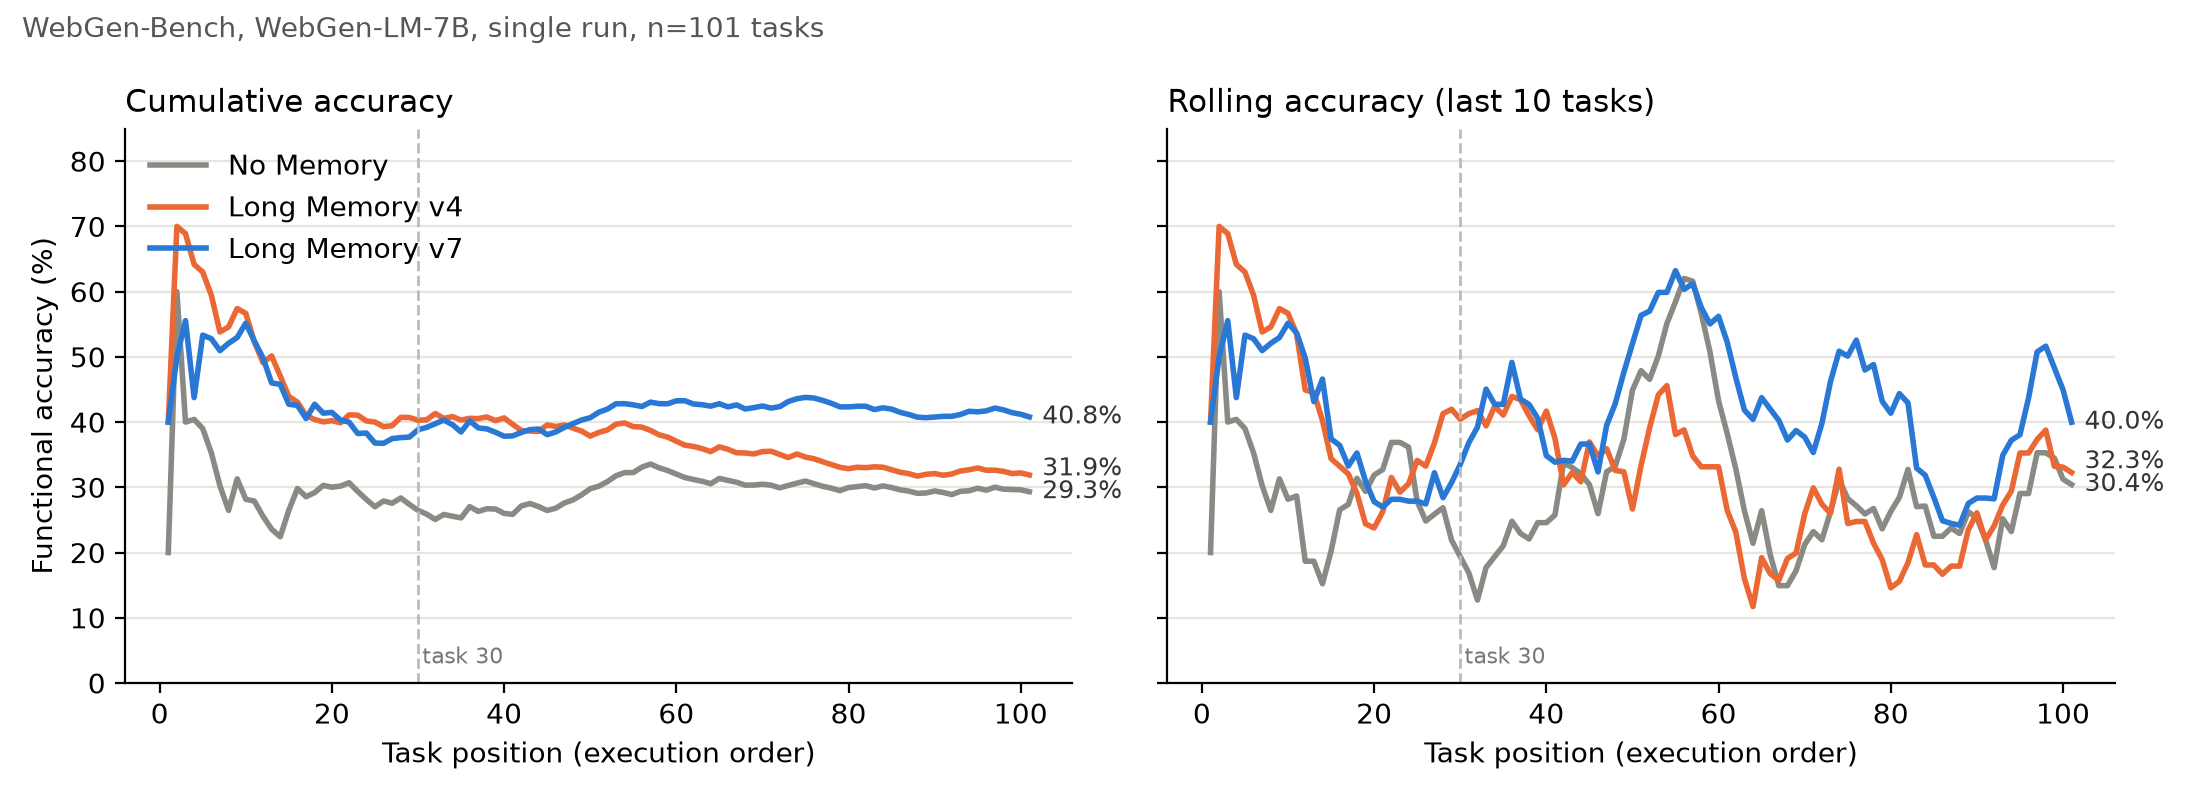
\includegraphics[width=\textwidth]{figures/learning_curve_v4_v7.png}
\caption{Cumulative and rolling-10 accuracy by execution order for No Memory, v4 and v7.}
\label{fig:curve}
\end{figure}

\Cref{fig:gap} shows the same data as a paired gap to No Memory. Both memories lead early; between tasks 40 and 60 v4 falls up to 27 points below No Memory while v7 stays near or above zero, and from task 60 onwards v7 stays clearly positive.

\begin{figure}[ht]
\centering
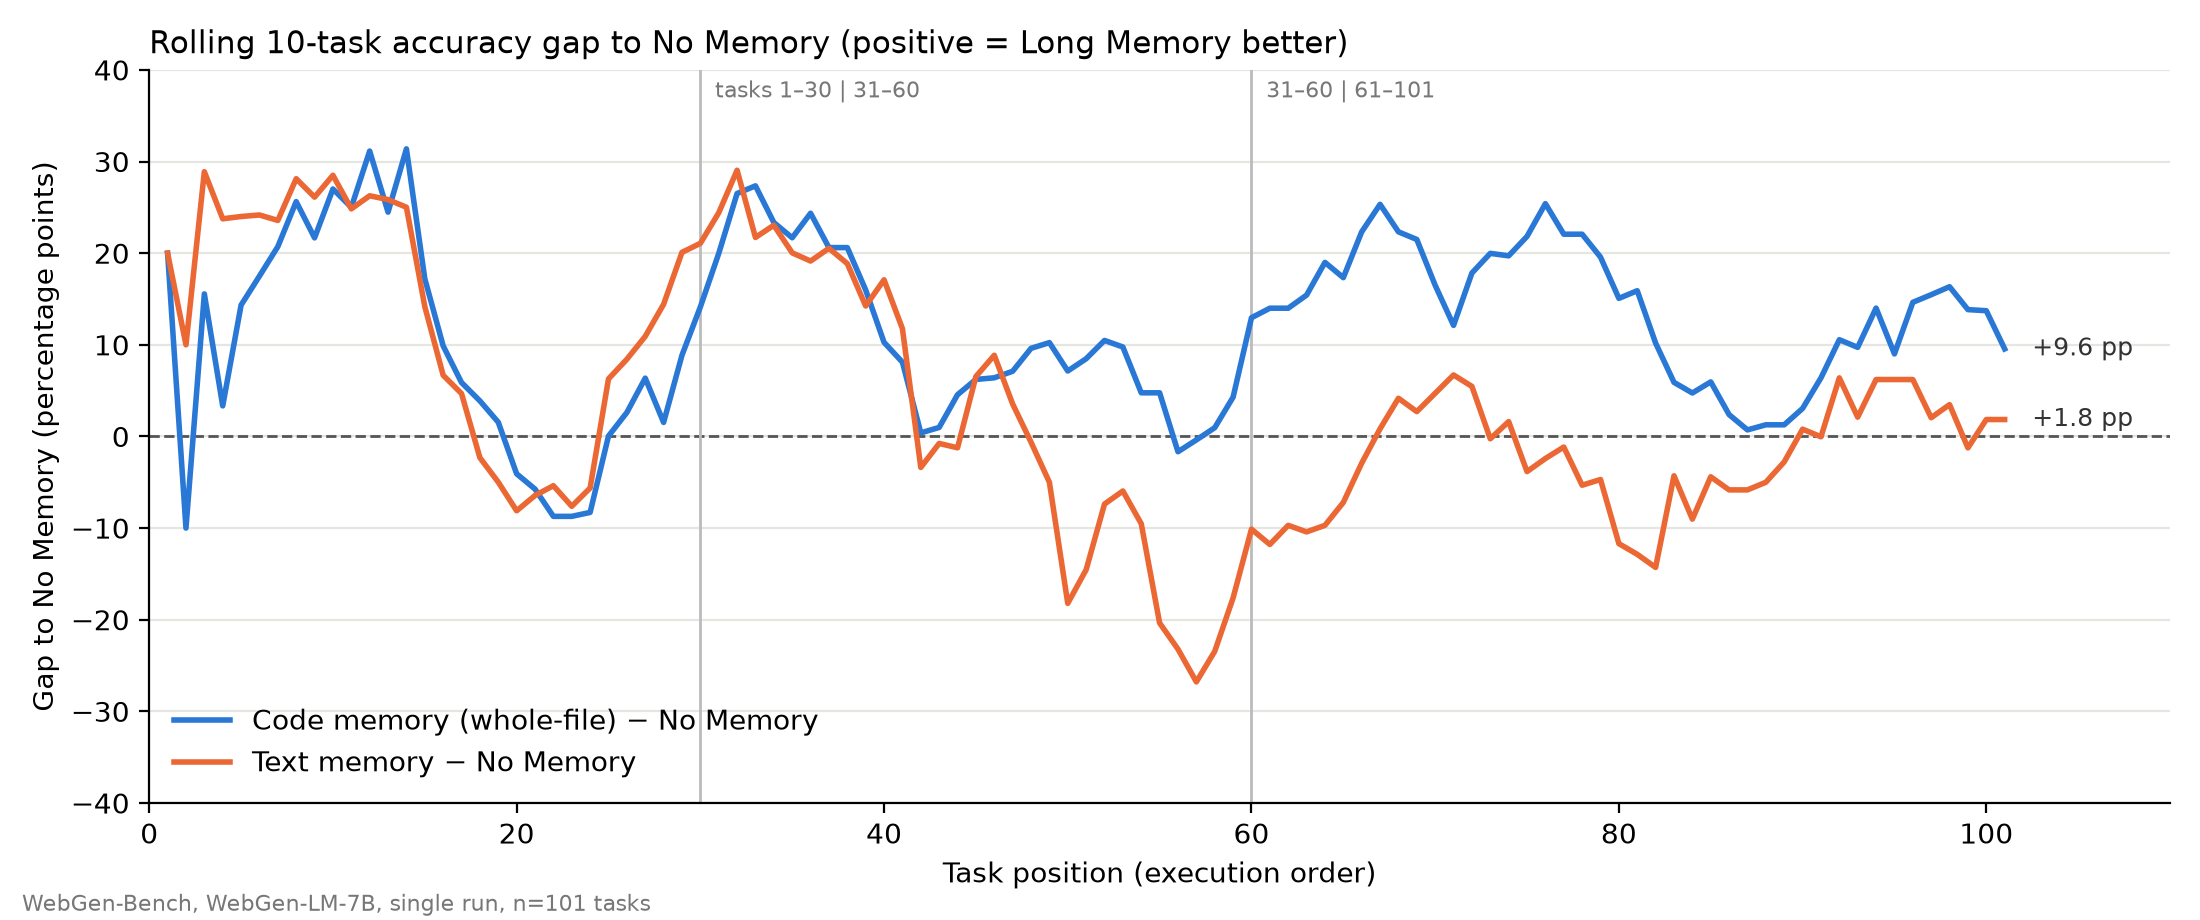
\includegraphics[width=\textwidth]{figures/gap_curve_v4_v7.png}
\caption{Rolling 10-task mean of the per-task accuracy gap to No Memory, by execution order. Positive values mean Long Memory is better.}
\label{fig:gap}
\end{figure}

\section{Why v4 Declines and v7 Improves}
\Cref{tab:prompt} counts what reached the generator's prompt, and \Cref{tab:codeerr} counts code problems in the generated sites, obtained by compiling every site with \texttt{@vue/compiler-sfc} 3.5.43. A lesson is counted as \emph{without a code construct} if it contains none of \texttt{@click}, \texttt{v-if}, \texttt{v-for}, \texttt{v-model}, \texttt{ref}, an \texttt{import} or inline code. In v4 such lessons appear in most tasks throughout and a separate ``General notes'' block becomes more frequent over time, while nothing addresses blank pages. In v7 these lessons are rarer and the code pool supplies a fragment in almost every task after it activates.

\begin{table}[ht]
\centering
\caption{Prompt content by segment (tasks 1--30 / 31--60 / 61--101).}
\label{tab:prompt}
\begin{tabular}{lcc}
\toprule
Prompt content & v4 & v7 \\
\midrule
Tasks with a lesson without a code construct & 23 / 25 / 28 & 12 / 4 / 11 \\
Tasks with a ``General notes'' block & 13 / 16 / 27 & 3 / 0 / 8 \\
Tasks with a code-pool fragment & 0 / 0 / 0 & 25 / 30 / 41 \\
Lessons attached to checklist items & 56 / 53 / 81 & 32 / 16 / 41 \\
\quad of which without a code construct (all tasks) & 102 of 190 & 31 of 89 \\
\bottomrule
\end{tabular}
\end{table}

\begin{table}[ht]
\centering
\small
\caption{Generated sites with code problems (number of tasks; 1--30 / 31--60 / 61--101, total in brackets).}
\label{tab:codeerr}
\begin{tabular}{lccc}
\toprule
Problem & No Memory & v4 & v7 \\
\midrule
Whole-site break\textsuperscript{a} & 11 / 5 / 10 (26) & 2 / 5 / 12 (19) & 4 / 1 / 3 (\textbf{8}) \\
Missing Vue import on a page & 7 / 7 / 9 (23) & 14 / 10 / 7 (31) & 12 / 4 / 6 (22) \\
\bottomrule
\multicolumn{4}{l}{\footnotesize \textsuperscript{a} An undeclared package import or a Vue compile error.}
\end{tabular}
\end{table}

These counts are correlational. Disentangling the contribution of each component requires the ablations in \Cref{sec:ablation}.

\section{Error Analysis}
Whole-site breaks fall from 26 tasks (No Memory) to 8 (v7), whereas pages with a missing Vue import are about as frequent as without memory (23 vs 22): the code pool prevents the error that blanks the whole site more reliably than the per-page one, which remains a basic error of the 7B generator. Counted per file, 27 of 592 generated Vue components in v7 (4.6\%) call a Vue function without importing it, against 27 of 586 (4.6\%) for No Memory. The omission occurs in \texttt{App.vue} and in child components alike, and is unrelated to whether a component uses \texttt{defineProps}/\texttt{defineEmits}; in the same file other imports are usually correct. It behaves like a random slip at a roughly constant per-file rate rather than a misconception, so a site with more components is more likely to contain one.

\paragraph{An attempted fix.} We tested a variant (v8) that rebuilds the code-pool example whenever the set of frequently missed functions changes, so that it shows both \texttt{ref} and \texttt{computed} (the v7 example was built at task 6 and only ever showed \texttt{ref}). Replacing only the code-pool section of the original v7 prompts, missing imports disappeared in one of four affected tasks and remained in the other three; two high-scoring regression tasks were unaffected. Because a random slip is not corrected by an example, and repairing generated code after generation is not allowed under the official protocol, we kept v7 as the final version and report this error rate as a limitation of the generator. Ten of v7's 13 zero-score tasks are also zero for No Memory, suggesting that most remaining failures are genuinely hard tasks for this generator.

Two v7 tasks returned the unmodified scaffold. A local diagnosis traced both to an example that was a complete \texttt{App.vue} file from another site; reducing it to a verified fragment restored real output on one task. This fix is not part of the frozen v7 run.

\paragraph{Appearance.} Restricted to the 68 tasks where both No Memory and v7 produced a working site with an appearance grade, the mean appearance score is 3.25 for No Memory and 3.22 for v7. The improvement is therefore functional; memory makes more sites work but does not make working sites look better.

\section{Ablation: Checklist Only}
\label{sec:ablation}
To separate the effect of requirement decomposition from that of memory, we run v7 with memory writes disabled, on the same task order. \todo{Fill in: Checklist-only accuracy / appearance / zero-score; contribution of checklist vs memory.}

\section{Robustness to Task Order}
\label{sec:order-design}
With memory, the order of tasks determines which experience is available, so a single order is not sufficient evidence. We therefore run Long Memory from an empty memory four times, each over all 101 tasks:
\begin{enumerate}
  \item the manifest (domain-block) order;
  \item a stratified shuffle with seed 11;
  \item a stratified shuffle with seed 29;
  \item a cross-domain interleaved order.
\end{enumerate}
In each order, Long Memory and No Memory are run as pairs on each task, alternating which arm runs first in an ABBA pattern, so that drift in infrastructure or evaluator load affects both arms equally. Results are reported per order as task-level paired differences with bootstrap \glspl{ci}, and by domain and position.

\begin{table}[ht]
\centering
\caption{Task-order experiments. \todo{Fill in when complete.}}
\label{tab:order}
\begin{tabular}{lcccc}
\toprule
Order & NM acc. & LM acc. & Paired diff. (95\% \gls{ci}) & Zero-score NM / LM \\
\midrule
Manifest & -- & -- & -- & -- \\
Shuffle (seed 11) & -- & -- & -- & -- \\
Shuffle (seed 29) & -- & -- & -- & -- \\
Interleaved & -- & -- & -- & -- \\
\bottomrule
\end{tabular}
\end{table}

\todo{Interpretation: stable gain in all orders (general benefit), gain only in domain blocks (curriculum effect), or worse when interleaved (cross-domain retrieval bottleneck).}

\chapter{Discussion}
\label{chap:discussion}

\section{The Role of Memory Representation}
Across the diagnostic and full runs, this small generator follows short code fragments more reliably than accumulated textual lessons. The text and code systems differ in more than representation, so this is a cross-version observation rather than a controlled causal comparison. It is consistent with Metis's finding that code memory can complement text memory~\cite{dai2026metis}, while adding a setting in which the format of the memory may determine whether a 7B generator can use it at all. The form of code also matters: complete files were sometimes copied as finished answers, whereas fragments prevented undeclared imports less reliably.

This pattern differs from reports for stronger models, which transfer text memory more reliably than code~\cite{dai2026metis,kim2026mtl}. The mechanisms are not identical because Metis executes code whereas this method displays code to the generator. Taken together, the evidence suggests that an appropriate memory representation depends on the capability of the model consuming it.

Part of the observed gain is protection against collapse rather than more capable application logic. In an early phase, short prompts led the model to return the default scaffold in five of eight tasks, whereas longer, specific prompts did not. Both effects can improve system performance, but they should be reported separately.

\section{What Is Learned and at What Cost}
The generator itself does not change. What changes is the code shown to it and the conditions under which it is shown. The resulting behaviour is closer to accumulating a small set of preventive code examples than to acquiring programming ability. It is also a property of the entire system, including a memory model that is larger than the generator. The memory remains small across 101 tasks; the study does not test what happens over thousands of tasks, when more problem types compete for three slots.

The system also adds computation. A Long Memory task takes approximately 12 minutes, compared with approximately 6 minutes for No Memory, largely because the 72B model constructs checklists, judges applicability, and reflects after each task. If the fixed-prefix ablation recovers most of the gain, a deployed system could use the learned fragments without invoking the 72B model at generation time, at the cost of losing online adaptation.

\section{Limitations and Threats to Validity}
\label{sec:threats}
\begin{itemize}
  \item \textbf{Single runs.} WebGen-Bench itself reports single runs without error bars. No Memory is repeated under several orders to estimate run-to-run noise, and Long Memory is repeated under further orders using paired comparisons. Within any order, however, Long Memory remains a single run. Two runs of the same Long Memory version can differ by approximately five points, which is more variation than observed for No Memory. The task-level intervals therefore understate full uncertainty. Orders share the same 101 tasks and are not independent samples. \todo{Status: a second manifest run of the final method is queued (about 10-19); report the difference between the two runs.}
  \item \textbf{Gain beyond the checklist and trade-offs between forms.} The final method's paired gain over checklist only is $+3.7$ [$-1.8$, 9.1], so an effect beyond requirement decomposition is not established. Whole-file examples also prevent undeclared imports more reliably in the original order, so neither code representation dominates everywhere.
  \item \textbf{One generator and one scaffold.} All results concern WebGen-LM-7B, Bolt.diy, and a Vue template. Larger generators may follow textual advice better and gain less from code examples.
  \item \textbf{Code pool as a learned prefix.} The general triggers make the code pool partly resemble a fixed prompt prefix. The fixed-prefix ablation (\Cref{sec:ablation}) is intended to measure how much of the effect this accounts for.
  \item \textbf{Rare problems are learned late.} A safeguard can appear only after the relevant problem has occurred. Memory may therefore help frequent problems more than rare ones, and several problem types can compete for three slots (\Cref{sec:fix}).
  \item \textbf{Evaluators.} Appearance uses Qwen2.5-VL-32B rather than GPT-4o and is therefore compared only across the present arms. \gls{gui} testers can exhaust their interaction budget or misjudge pages~\cite{zheng2023judge}. Raw transcripts are retained, but the judgements were not independently reviewed by a human.
  \item \textbf{Iterative development on the same benchmark.} This is the most serious limitation. Every version was designed after failures were observed on the same 101 tasks used for evaluation. The effect is visible: whole-file code memory, developed on the manifest order, scores 40.0\% there but 33.1\% and 32.6\% in the two shuffled orders, while No Memory stays at 27.9--28.6\%. Empty memories and freezing the final version before all runs except seed 11 reduce this risk but do not remove it. A held-out evaluation is required.
  \item \textbf{Memory model stronger than generator.} The 72B memory model exceeds the 7B generator in size, so some gains may reflect the larger model's organisation of the task. The checklist only restates the requirement, every fragment is copied verbatim from an earlier site generated by the 7B model, and the memory model never sees the current task's evaluation. The results therefore concern what a small generator gains when a stronger model organises its prior experience, rather than self-improvement in isolation. \todo{Status: fixed-prefix run queued after seed 47. State how much of the gain remains without accumulated memory and without the 72B model at generation time.}
\end{itemize}

\section{Ethical Considerations and Impact}
\paragraph{Data and privacy.} The benchmark requirements are synthetic and contain no personal data. All models run on university hardware, and no task data are sent to external services.
\paragraph{Environmental cost.} A full run occupies two H200 GPUs for about one day (\Cref{sec:design}). To limit unnecessary computation, changes were first checked on three to five tasks and with static code analysis before full evaluation.
\paragraph{Self-improving agents and society.} A memory system that turns outcomes into later behaviour can preserve mistakes as readily as useful practices. This design retains provenance for every memory entry so that injected material can be traced, but systems that store and reuse code in deployment would still require security review. Small local models can reduce website-development costs for smaller organisations, while potentially displacing routine front-end work. Their output remains subject to human review.
\paragraph{Use of AI tools.} Claude and ChatGPT were used to assist with programming the experimental pipeline and analysis scripts, organising experiment logs, and giving suggestions in critical reviews of drafts; Gemini and Microsoft Copilot were also used for review comments. All text was written by the author, who decided which suggestions to adopt. Research decisions and the verification of all results are the author's responsibility; every number was computed by the scripts in the public repository and checked by the author. \todo{Author: this statement holds only after the final text has been rewritten in your own words; check it against what was actually done before submission.}

\paragraph{Research integrity.} We report negative results (text memory's decline, the scaffold failure of whole-file examples) and invalidated our own earlier results when a delivery bug was found.

\section{Project Management}
The project was organised in versions. The cluster ran one frozen version at a time; new ideas were tested locally on small samples and with static code checks, and a version was replaced only when the new one was shown to be better. Decisions and their evidence were recorded continuously in a decision log, which made it possible to reconstruct why each component exists.

\chapter{Conclusion}
\label{chap:conclusion}

\section{Answers to the Research Questions}
\paragraph{\ref{rq1}} A qualified yes, for WebGen-LM-7B with Bolt.diy on WebGen-Bench. The final code memory raises accuracy from 28.5\% to 35.2\% (+7.1, CI excludes zero) and cuts zero-score tasks from 30 to 20, with gains of 7.4 and 5.5 points in two shuffled orders; most of the gain comes from sites that now render. \todo{Status: summarise all orders once seed 47 and interleaved finish.}

\paragraph{\ref{rq2}} The small generator followed short code fragments from its own earlier websites but rarely followed textual lessons; text memory fell behind No Memory late in the sequence (a cross-version, not controlled, comparison). The checklist alone added little (+3.4, interval includes zero). Fragments must be partial: a complete file was copied as a finished answer. \todo{Status: add the fixed-prefix result (queued after seed 47).}

\paragraph{\ref{rq3}} Code memory keeps its advantage over the sequence (35.3\% vs 29.5\% on tasks 31--101) while text memory declines, consistent with, but not proof of, learning from experience. Whole-file examples caused scaffolds when the order changed; with verified fragments the scaffolds disappeared and the gain was positive in both kinds of order, though robustness is not yet established. The whole-file design scored higher only in the original order (40.0\%). \todo{Seed 47 and interleaved order with the final method.}

\section{Future Work}
Two further experiments would address the main remaining questions:
\begin{itemize}
  \item \textbf{Held-out evaluation.} Because the method was developed while observing results on all 101 tasks, a clean test needs tasks that were never seen: a held-out domain, or a second website-generation benchmark, with the method frozen beforehand.
  \item \textbf{Controlled form-of-memory comparison.} Keep retrieval, trigger and token budget fixed and vary only the form: textual rule, pseudocode, short fragment, complete file, plus random-code and length-matched text controls.
\end{itemize}
Further directions are repeating each order more than once, to separate order effects from run-to-run variation, and testing larger generators of the same family, with a text-memory arm, to see whether the preference for code depends on model size.


\backmatter
\bibliographystyle{plain}
\bibliography{bibliography}

\end{document}
